\section{ Conceptos generales de árboles }
\subsection{La teoría de grafos y los árboles}
El concepto de \textbf{árbol} como estructura de datos tiene su origen en el
concepto de grafo.  Repasando, a continuación algunos conceptos de
grafos:

\begin{itemize}
\item \textbf{Grafo}: es una colección de de vértices $V$, y una
  colección de lados $L$, donde por cada lado en $L$, hay una línea
  que une un par de vértices en $V$
\item \textbf{Vértices Adyacentes}: son los que están unidos por un
  lado
\item \textbf{Ruta}: de longitud $n$, es una secuencia de lados $l_1
  l_2 \dotso l_n$, donde lado $l_k$ comparte un vértice en común con
  el lado precedente $l_{k-1}$, y un vértice en común con el lado
  subsiguiente $l_{k+1}$, para $1 < k < n$. Otra definición es: Ruta
  de longitud $n$ es un conjunto de vértices $v_0v_1 \ldots v_n$, tal
  que $v_{k-1}$ es adyacente a $v_k$, para $1 < k < n$.
\item \textbf{Ruta Simple}: cuando todos los vértices en él son
  distintos, excepto posiblemente por el primero y último
\item \textbf{Ciclo}: es una ruta de longitud tres o más, que conecta
  un vértice $v$ con él mismo.
\item \textbf{Ciclo Simple}: es un ciclo, cuya ruta es simple.
\item \textbf{Grafo Conectado}: es aquel donde existe, al menos una
  ruta de un vértice a otro.
\item \textbf{Árbol libre}: es un grafo finito y conectado, sin ciclos
  simples.
\item \textbf{Árbol orientado}: es un grafo, donde cada lado de $L$,
  es un par de vértices de la forma $(v, v’)$ donde se dice que $v$ es
  el origen y $v’$ es el destino y la dirección de $l$ va de $v$ a
  $v’$, y se toma un vértice $r$ como la raíz donde inicia el grafo.
\item \textbf{Árbol ordenado}: es un conjunto finito de uno o más
  vértices tales que hay un vértice designado $r$, llamado la raíz, y
  tal que los vértices restantes, son divididos en $n > 0$
  subconjuntos mutuamente exclusivos, cada uno de los cuales son a la
  vez árboles ordenados.
\item \textbf{Árbol binario}: Es un conjunto finito de vértices que
  están vacíos o consiste de un vértice llamado raíz y dos subárboles
  binarios, los cuales son disjuntos uno del otro, y son llamados
  subárboles izquierdo y derecho
\item \textbf{Árbol binario lleno}: Es un árbol binario en el cual
  cada nodo o es hoja o tiene exactamente dos descendientes no vacíos.
\item \textbf{Árbol binario completo}: es un árbol binario con hojas
  en los dos últimos niveles y en las hojas del último nivel están a
  la izquierda
\end{itemize}

Los árboles como estructuras de datos son sólo una de las aplicaciones
que existen para este concepto.  Entre ellos están los \textbf{árboles de
costo mínimo}, los \textbf{árboles de expresiones}, \textbf{mapas}, etc.

\subsection{Representaciones de árboles en memoria}
\label{sec:repr-de-arbol}

Los árboles binarios son construidos típicamente con una estructura de
nodos y apuntadores en la cual se almacenan datos, cada uno de estos
nodos tienen una referencia o apuntador a un nodo izquierdo y a un
nodo derecho denominados hijos. En ocasiones, también contiene un
apuntador a un único nodo. Si un nodo tiene menos de dos hijos,
algunos de los punteros de los hijos pueden ser definidos como nulos
para indicar que no dispone de dicho nodo. En la figura adjunta se
puede observar la estructura de dicha implementación.

\begin{figure}[H]
  \centering
  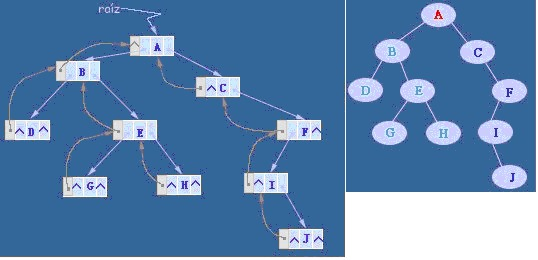
\includegraphics[scale=.5]{1arbolEnMemoria.jpg}
  \caption{Árbol en memoria}
  \label{fig:1arbolEnMemoria}
\end{figure}

Los árboles binarios también pueden ser almacenados como una
estructura de datos implícita en arrays, y si el árbol es un árbol
binario completo, este método no desaprovecha el espacio en
memoria. Tomaremos como notación la siguiente: si un nodo tiene un
índice $i$, sus hijos se encuentran en índices $2i+1$ y $2i + 2$,
mientras que sus padres (si los tiene) se encuentra en el índice
$(i-1)/2$ (partiendo de que la raiz tenga índice cero). Este método
tiene como ventajas el tener almacenados los datos de forma más
compacta y por tener una forma mas rápida y eficiente de localizar los
datos en particular durante un preoden transversal. Sin embargo, \textit{si el
árbol no está completo, desperdicia mucho espacio en memoria}.
\begin{figure}[H]
  \centering
  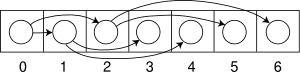
\includegraphics[scale=.7]{2arbolBinarioEnArray.jpg}
  \caption{Árbol binario en array.}
  \label{fig:2arbolBinarioEnArray}
\end{figure}

\subsection{Codificación de árboles n-arios como árboles binarios}
\label{sec:codif-de-arbol}
Hay un mapeo uno a uno entre los arboles generales y arboles binarios,
el cual en particular es usado en Lisp para representar arboles
generales como arboles binarios. Cada nodo $N$ ordenado en el árbol
corresponde a un nodo $N'$ en el árbol binario; el hijo de la
izquierda de $N'$ es el nodo correspondiente al primer hijo de $N$, y
el hijo derecho de $N'$ es el nodo correspondiente al siguiente
hermano de $N$, es decir, el próximo nodo en orden entre los hijos de
los padres de $N$.

Este representación de árbol binario de un árbol general, a veces se
hace referencia como un árbol binario \textbf{primer hijo/siguiente hermano}, o
un árbol doblemente encadenado.

Una manera de pensar acerca de esto es que los hijos de cada nodos
esten en una lista enlazada, encadenados junto con campo derecho, y el
nodo sólo tiene un \textbf{apuntador} al comienzo o la cabeza de esta
lista, a través de su campo izquierdo.

Por ejemplo, en el árbol de la izquierda, la A tiene 6 hijos (B, C, D,
E, F, G). Puede ser convertido en el árbol binario de la derecha.
\begin{figure}[H]
  \centering
  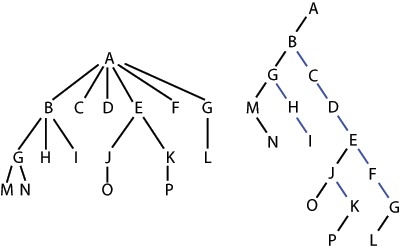
\includegraphics[scale=2]{3arbolGeneralABinario.jpg}
  \caption{Árbol general a binario}
  \label{fig:3arbolGeneralABinario}
\end{figure}

Esta representación tiene la ventaja que puede representar cualquier
árbol multihijos, utilizando sólo dos apuntadores por nodo.  Es útil
cuando el árbol a representar tiene una gran cantidad de hijos por
nodo, o la cantidad de hijos es variable y/o indeterminada.

La desventaja es que los recorridos se complica.

\section{Operaciones sobre árboles}
\label{sec:oper-sobre-arbol}

Como estructura de datos, sobre los árboles se pueden realizar
diferentes operaciones como agregar, buscar y eliminar elementos del
árbol.  Sin embargo cualquier problema que se quiera resolver con el
uso de árboles, en general, se convertirá en realizar un
\textbf{recorrido} sobre el árbol.

\subsection{Recorridos}
\label{sec:recorridos}
\begin{definicion}
  Un \textbf{recorrido} es una operación sobre un árbol en el que se
  recorren los elementos en algún orden definido, para realizar sobre
  los elementos algún proceso, llamado VISITA.
\end{definicion}

Según esta definición, hay $n!$ formas de recorrer un árbol con n
elementos, lo cual nos deja un número igual de recorridos posibles.
Sin embargo, las operaciones de recorrido definidas se refieren
normalmente a \textbf{recorridos completos}.

\begin{definicion}
  Un \textbf{recorrido completo} es un tipo de recorrido en el cual se
  VISITAN todos elementos del árbol, en algún orden definido.
\end{definicion}


Existen varios recorridos definidos, pero veremos cuatro principales.
Así, sea un árbol T con subarbol izquierdo Ti y subarbol derecho Td,
entonces se tienen los siguientes recorridos

\begin{description}
\item[Preorden: ] es el recorrido donde se VISITA T y luego se realiza
  el recorrido preorden de Ti y luego el recorrido preorden de Td
\item[En orden: ] es el recorrido donde se realiza el recorrido en
  orden de Ti, y luego se VISITA T y luego el recorrido en orden de Td
\item[Postorden: ] es el recorrido se realiza el recorrido post orden
  de Ti, luego el recorrido post orden de Td y luego se VISITA T
\item[Por niveles: ] es el recorrido donde se VISITAN los nodos en el
  orden del nivel del árbol, así se visita T, luego se realiza el
  recorrido de las raices de Ti y Td, luego el recorrido por nivel de
  los hijos inmediatos de Ti y Td, y así sucesivamente hasta recorrer
  todos los niveles.
\end{description}

Cada uno de estos recorridos produce una secuencia de elementos que
toma el nombre del recorrido correspondientes.  Así hablamos de la
\textit{secuencia preorden}, \textit{secuencia en orden}, etc.
Por ejemplo: en el siguiente árbol
\begin{figure}[H]
  \centering
  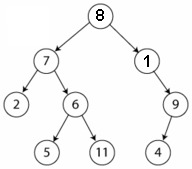
\includegraphics[scale=.6]{4arbolSecuencias.jpg}
  \caption{Secuencias de un árbol.}
  \label{fig:4arbolSecuencias}
\end{figure}

Tiene las siguientes secuencias:


\begin{itemize}
\item Secuencia pre orden: 8, 7, 2, 6, 5 , 11, 1, 9, 4
\item Secuencia en orden: 2, 7, 5, 6, 11, 8, 1, 4, 9
\item Secuencia post orden: 2, 5, 11, 6, 7, 4, 9, 1, 8
\item Secuencia por niveles: 8, 7, 1, 2, 6, 9, 5, 11, 4
\end{itemize}

En cada secuencia de llaves, que determina una relación de sucesor y
predecesor en cada recorrido, así hablamos de relaciones
sucesor-predecesor, según las secuencias.  Por ejemplo: 5 es
predecesor en preorden del 11, predecesor en orden del 6, sucesor en
postorden del 2

Una posible implementación es:

\begin{verbatim}
class NodoBin {
   NodoBin *izq ;
   NodoBin *der ;
   TInfo info ;
   .....
}

class ArbolBinario {
   public:
      void preOrden () {
         preOrden(raiz) ;
      }

      void enOrden () {
         enOrden(raiz) ;
      }


      void postOrden () {
         postOrden(raiz) ;
      }
   private:
      NodoBin *raiz ;
      ....
      void visita (NodoBin *n) {
          // cualquier operación que se desee hacer sobre cada nodo
      }

      void preOrden (NodoBin *n) {
         if  ( n != null) {
            visita (n) ;
            preOrden(n->izq) ;
            preOrden(n->der) ;
         }
      }

      void enOrden (NodoBin *n) {
         if  ( n != null) {
         enOrden(n->izq) ;
         visita (n) ;
         enOrden(n->der) ;
         }
      }

      void postOrden (NodoBin n) {
         if  ( n != null) {
            postOrden(n->izq) ;
            postOrden(n->der) ;
            visita (n) ;
         }
      }
} 
\end{verbatim}

\section{Árboles binarios de búsqueda}
\label{sec:arboles-binarios-de}

Un árbol de búsqueda, también de comparación o decisión, es un árbol
en el que cada llave $L$ tiene subárbol izquierdo y derecho, tal que las
llaves del subárbol izquierdo de $L$ son menores a $L$, y las del subárbol
derecho son mayores a $L$, y los subarboles derecho e izquierdo de $L$ son
también árboles de búsqueda.

Nótese que hablamos de llaves en vez de nodos

\subsection{Árbol binario de búsqueda}
\label{sec:arbol-binario-de}
Es un árbol de búsqueda en el que cada nodo tiene si mucho 2 hijos.

Por ejemplo, en la siguiente gráfica tenemos el árbol binario
anterior, convertido en árbol binario de búsqueda:

\begin{figure}[H]
  \centering
  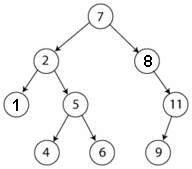
\includegraphics[scale=0.5]{5arbolBusquedaBinaria.jpg}
  \caption{Árbol binario de busqueda de Figura \ref{fig:4arbolSecuencias}}
  \label{fig:5arbolBusquedaBinaria}
\end{figure}

 Otro ejemplo:
\begin{figure}[H]
  \centering
  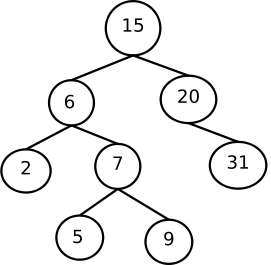
\includegraphics[scale=0.4]{6otroArbolBusquedaBinaria.jpg}
  \caption{Otro árbol binario de busqueda.}
  \label{fig:6otroArbolBusquedaBinaria}
\end{figure}

\subsection{Búsqueda}
\label{sec:busqueda}

La búsqueda consiste acceder a la raíz del árbol, si el elemento a
localizar coincide con éste la búsqueda ha concluido con éxito, si el
elemento es menor se busca en el subárbol izquierdo y si es mayor en
el derecho. Si se alcanza un nodo hoja y el elemento no ha sido
encontrado se supone que no existe en el árbol. Cabe destacar que la
búsqueda en este tipo de árboles es muy eficiente, representa una
función logarítmica de base 2.
\begin{verbatim}
class NodoBin {
   TLlave llv ;
   TValor value
   NodoBin *izq, *der ;

   NodoBin (TLlave llv, TValor value) {
      this->llv = llv ;
      this->value = value ;
      izq = null ;
      der = null ;
   }
}

class ArbolBinBusqueda :: ArbolBinario {
   NodoBin *raiz ;
   .....
   TValor get(TLlave llv) {
      NodoBin * temp = raiz ;

      while ( temp != nullptr && llv != temp.llv) {
         if (llv < temp->llv) {
            temp = temp->izq ;
         }else{
            temp = temp->der ;
         }
      }

      if ( temp == null)
          return null ; // no está
      else
          return temp.valor ;
   }
} 
\end{verbatim}

\textbf{Uso correcto de clases}: En general, cuando trabajamos
programación orientada a objetos, se comete el error común de
saltarnos un método de una clase.  Usualmente tenemos un método como
el siguiente:
\begin{verbatim}
class x {
   ....
   int x1(T obj) {
      if ( obj.a() )
          x = obj.b() ;
      ....
      obj.c() ;
      ..
      obj.d() ;
      ..
   }
   ...
   int y() {
      ...
      x1(o) ;
      ..
   }
} 
\end{verbatim}

Nos damos cuenta que en el método \textbf{x1}, se se recibe un
parámetro del clase \textbf{T}, y toda la lógica del método es
alrededor de dicho parámetro (\textbf{obj}), entonces ésto debería
convertirse en:
\begin{verbatim}
class T {
   int x1() {
      if (a() ) ..
         x = b() ;
      c() ;
      ..
      d() ;
      ..
   }
   ....
}

class x {
   ...
   int y() {
      ...
      o.x1() ;
      ..
   }
}
\end{verbatim}

\subsection{Orden de la búsqueda}
\label{sec:orden-de-la}

\begin{eqnarray*}
  \label{eq:1}
  T(get(n)) &=& T(asignacion) + T(while) + T(if) ;\\
    &=& t + ( T(condicion) + K * T(cuerpo) ) + ( T(condicion) + max ( T(then) , T(else) )  )\\
    &=& t + ( t + K ( T(if) ) ) + ( t + max ( t, t ) ) \\
    &=& t + ( t + K ( T(condicion) + max ( T(then) , T(else) )) ) + ( t +  t ) \\
    &=& t + ( t + K ( t + max ( t , t )) ) + ( t +  t ) \\
    &=& t + ( t + K ( t + t ) + ( t +  t ) 
\end{eqnarray*}

$K$ es el número de veces que se ejecuta el cuerpo del while, en
términos de $n$, donde $n$ es el número de llaves.

$K$ = altura del arbol y la relación entre la altura y $N$ está dada por  
\[ 2^k - 1 = n  \longrightarrow   k = lg ( n + 1)\]

por lo tanto
\begin{eqnarray*}
  \label{eq:2}
  T(get(n)) &=&  t + ( t + lg ( n + 1) ( t + t ) + ( t +  t ) \\
    &=& 4t + lg ( n + 1) ( 2t + t ) \longrightarrow O(get(n)) = lg(n) 
\end{eqnarray*}

\subsection{Inserción}
\label{sec:insercion}

La inserción es similar a la búsqueda. Se procede de la siguiente
forma, si el nodo pasado como parámetro está vacío se crea un nuevo
nodo para él cuyo contenido correspondiente sería el elemento a
insertar. Si no lo está, se comprueba si el elemento dado es menor que
el de la raíz del árbol con lo que se inserta en el subárbol
izquierdo, o mayor, insertándose en el subárbol derecho. Se observa
que de este modo las inserciones se realizan en las hojas, es la forma
más simple de llevar a cabo esta tarea, aunque no la única.
\begin{figure}[H]
  \centering
  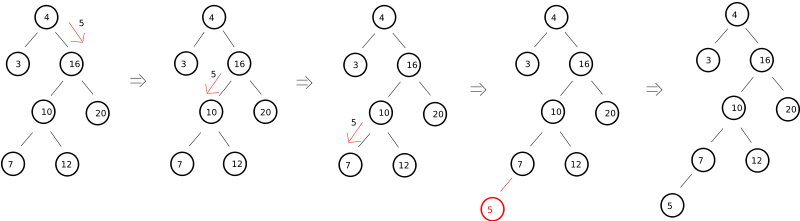
\includegraphics[scale=.45]{7arbolInsercion.jpg}
  \caption{Insercion en árbol}
  \label{fig:7insercion}
\end{figure}

\subsection{Eliminación}
\label{sec:eliminacion}

La operación de borrado no es tan sencilla como las de búsqueda e
inserción. Existen varios casos a tener en consideración:
\begin{itemize}
\item Borrar un nodo sin hijos ó nodo hoja: simplemente se borra y se
  establece a nulo el apuntador de su padre.
\item Borrar un nodo con un subárbol hijo: se borra el nodo y se
  asigna su subárbol hijo como subárbol de su padre.
\item Borrar un nodo con dos subárboles hijo: la solución está en
  reemplazar el valor del nodo por el de su predecesor o por el de su
  sucesor en orden y posteriormente borrar este nodo. Su predecesor en
  orden será el nodo más a la derecha de su subárbol izquierdo (mayor
  nodo del subarbol izquierdo), y su sucesor el nodo más a la
  izquierda de su subárbol derecho (menor nodo del subarbol
  derecho). En la siguiente figura se muestra cómo existe la
  posibilidad de realizar cualquiera de ambos reemplazos:
\end{itemize}
\begin{figure}[H]
  \centering
  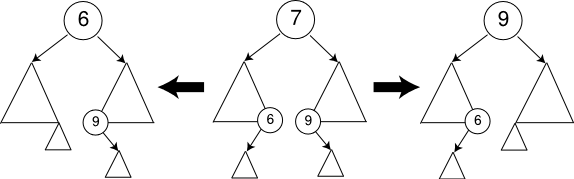
\includegraphics[scale=.55]{8arbolEliminacion.jpg}
  \caption{Eliminación en árbol}
  \label{fig:8arbolEliminacion}
\end{figure}

\begin{verbatim}
class ArbolBinBusqueda:: ArbolBinario {
public:
   ....
   TValor remove(TLlave key) {
      return remove (raiz, key) ;
   }

   TValor remove (NodoBin *n, TLlave key) {
      TValor value = null ;
      NodoBin *padre = null ;

      while (n != nullptr && n->llave != key) {
         padre = n ;
         if (key < n->llave)
            n=n->izq ;
         else
            n = n->der ;
      }

      if (n!=nullptr) {
         value = n->value ;
         if (n->izq == null && n->der == nullptr) { //es nodo hoja
            if (padre->izq == n)
               padre->izq = null ;
            else
                padre->der = null ;
         }else{
            if (n->izq == null) { // sólo tiene hijo derecho
               if (padre->izq == n)
               padre->izq = n->der ;
            else
               padre->der = n->der ;
         }else{
            if (n->der == nullptr) { // sólo tiene hijo izquierdo
               if (padre->izq == n)
                  padre->izq = n->izq ;
               else
                  padre->der = n->izq ;
         }else{ // tiene dos subárboles
            // predecesor en orden
            NodoBin *temp = n->izq ;
            while (temp->der != nullptr)
               temp = temp->der ;
            n->llave = temp->llave ;
            n->valor = temp->valor ;
            remove (n->izq, n->llave) ;
         }//if interno
      }//if
      return value ;
   }//funcion remove
}
\end{verbatim}

En el caso ideal una búsqueda de una llave tiene un orden $O(n)=lg (n)$,
sin embargo puede suceder el fenómeno del desbalance

\subsection{Árbol AVL}
\label{sec:arbol-avl}

El árbol AVL toma su nombre de las iniciales de los apellidos de sus
inventores, Adelson-Velskii y Landis. Lo dieron a conocer en la
publicación de un artículo en 1962: <<An algorithm for the organization
of information>> (<<Un algoritmo para la organización de la
información>>).

Los árboles AVL están siempre equilibrados de tal modo que para todos
los nodos, la altura de la rama izquierda no difiere en más de una
unidad de la altura de la rama derecha. Gracias a esta forma de
equilibrio (o balanceo), la complejidad de una búsqueda en uno de
estos árboles se mantiene siempre en orden de complejidad O(lg n). El
factor de equilibrio puede ser almacenado directamente en cada nodo o
ser computado a partir de las alturas de los subárboles.

Para conseguir esta propiedad de equilibrio, la inserción y el borrado
de los nodos se ha de realizar de una forma especial. Si al realizar
una operación de inserción o borrado se rompe la condición de
equilibrio, hay que realizar una serie de rotaciones de los nodos.

Los árboles AVL más profundos son los árboles de Fibonacci.

\subsubsection{Definición.}
\label{sec:definicion}
\begin{definicion}
  \textbf{Altura de un árbol}.  Sea T un árbol binario de búsqueda y sean Ti y
  Td sus subárboles, su altura H(T), es:
  \begin{itemize}
  \item 0 si el árbol T está vacío
  \item 1 + max(H(Ti),H(Td)) si no está vacío
  \end{itemize}
\end{definicion}

\begin{definicion}
  \textbf{Árbol AVL}.  Sea T un árbol binario de búsqueda (ABB) con Ti
  y Td siendo sus subárboles izquierdo y derecho respectivamente,
  tenemos que:
  \begin{itemize}
  \item Si T es vacío, es un árbol AVL
  \item Si T es un ABB no vacío, es AVL si (si y sólo si):
    \begin{itemize}
    \item[*] Ti y Td son AVL y
    \item[*] -1 <= H(Ti) - H(Td) <= 1
    \end{itemize}
  \end{itemize}
\end{definicion}

Ej: árbol binario de búsqueda desbalanceado
\begin{figure}[H]
  \centering
  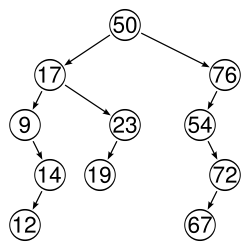
\includegraphics[scale=0.5]{9arbolBinBusquedaDesbalanceado.jpg}
  \caption{Árbol binario de búsqueda desbalanceado}
  \label{fig:9arbolBinBusquedaDesbalanceado.jpg}
\end{figure}

Mismo árbol balanceado
\begin{figure}[H]
  \centering
  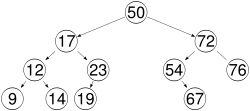
\includegraphics[scale=0.5]{10arbolBinBusquedaBalanceado.jpg}
  \caption{Árbol binario de búsqueda balanceado}
  \label{fig:10arbolBinBusquedaBalanceado}
\end{figure}
Por esta definición tenemos que el árbol de la figura de arriba no es
AVL, mientras que el de abajo sí lo es. Véase también que se trata de
un árbol ordenado, en el cual para cada nodo todos los nodos de su
subárbol izquierdo tienen un valor de clave menor y todos los nodos de
su subárbol derecho tienen un valor de clave mayor que el suyo,
cumpliendo así la propiedad de los ABB.

\subsubsection{Factor de equilibrio}
\label{sec:factor-de-equilibrio}

Cada nodo, además de la información que se pretende almacenar, debe
tener los dos apuntadores a los árboles derecho e izquierdo, igual que
los árboles binarios de búsqueda (ABB), y además el dato que controla
el factor de equilibrio.

El factor de equilibrio es la diferencia entre las alturas del árbol
derecho y el izquierdo:

FE = altura subárbol derecho - altura subárbol izquierdo;

Por definición, para un árbol AVL, este valor debe ser -1, 0 ó 1.

\subsubsection{Operaciones}
\label{sec:operaciones}

Las operaciones básicas de un árbol AVL implican generalmente el
realizar los mismos algoritmos que serían realizados en un árbol
binario de búsqueda desequilibrado, pero precedido o seguido por una o
más de las llamadas <<rotaciones AVL>>.

\paragraph{Búsqueda}
\label{sec:busqueda-1}

Las búsquedas se realizan de la misma manera que en los ABB, pero al
estar el árbol equilibrado la complejidad de la búsqueda nunca
excederá de O(log n).

\begin{verbatim}
class NodoAVL::NodoBin {
   int balance ;
   NodoAVL(TLlave llv, TValor value):NodoBin (llv,value) {
      balance = 0 ;
   }

   NodoAVL *rotacionDer() {
      NodoAVL *temp = izq ;
      izq = izq.der ;
      temp.der = this ;
      return temp ;
   }
}

class ArbolAVL::ArbolBinarioBusqueda {
   private:
      NodoAVL<K,V> raiz ;
   public:
      .....
      TValor get(TLlave llv) {
         NodoBin *temp = raiz ;
         while (temp != nullptr && llv != temp->llv) {
            if (llv < temp>llv) {
               temp = temp.izq ;
            }else{
               temp = temp.der ;
            }
         }
         if (temp == nullptr)
            return nullptr ; // no está
         else
            return temp.valor ;
      }
      .....
}
\end{verbatim}

\paragraph{Inserción}
\label{sec:insercion-1}

La inserción en un árbol de AVL puede ser realizada insertando el
valor dado en el árbol como si fuera un árbol de búsqueda binario
desequilibrado y después retrocediendo hacia la raíz, rotando sobre
cualquier nodo que pueda haberse desequilibrado durante la inserción.

Dado que como mucho un nodo es rotado 1.5 veces log n en la vuelta
hacia la raíz, y cada rotación AVL tarda el mismo tiempo, el proceso
de inserción tarda un tiempo total de O(log n).

\begin{verbatim}
class ArbolAVL::ArbolBinarioBusqueda {
   private:
      NodoAVL *raiz ;
   public:
   .....
   TValor put (TLlave llv, TValor value) {
      bool crecio= false ;
      if (raiz == nullptr) // árbol vacío
         raiz = new NodoAVL(llv, value) ;
      else
         raiz = put(llv, value, raiz, crecio) ;
      return value ;
   }
   NodoAVL *put (TLlave llv, TValor value, NodoAVL *n, bool &crecio) {
      if (llv == n->llv) // ya está ==> error
         throw "Duplicado" ;
      else if (llv < n->llv) { // debe insertarse a la izquierda
         if (n->izq != null) {  // existe hijo izquierdo
            put (llv, value, n->izq, crecio) ;
            if ( crecio ) {
               n->balance -- ;
               if (n->balance < -1) { //necesario balancear
                  if ( n->izq->balance > 0 ) //rotación doble
                     n->izq = n->izq->rotacionIzq() ;
                  crecio = false ;
                  return n->rotacionIzq() ;
               }
            }
         }else{ // no existe hijo izquierdo
            n->izq = new NodoAVL(llv, value) ;
            n.balance -- ;
            crecio = (n.balance!=0) ;
         }
      }else{  // debe insertarse en la derecha
         if (n->der != nullptr) { // existe hijo derecho
            put (llv, value, n->der, crecio) ;
            if ( crecio ) {
               n->balance ++ ;
               if (n->balance > 1) { //necesario balancear
                  if ( n->der->balance < 0 ) //rotación doble
                     n->der = n->der->rotacionDer() ;
                  crecio = false ;
                  return n->rotacionIzq() ;
               }
            }
         }else { //no existe hijo derecho
            n->der = new NodoAVL(llv, value) ;
            n.balance ++ ;
            crecio = (n->balance!=0) ;
         }
     }
} 
\end{verbatim}

\paragraph{ Extracción}
\label{sec:extraccion}

El problema de la extracción puede resolverse en O(log n) pasos. Una
extracción trae consigo una disminución de la altura de la rama donde
se extrajo y tendrá como efecto un cambio en el factor de equilibrio
del nodo padre de la rama en cuestión, pudiendo necesitarse una
rotación.

Esta disminución de la altura y la corrección de los factores de
equilibrio con sus posibles rotaciones asociadas pueden propagarse
hasta la raíz.

\subsection{Árbol HB[K]}
\label{sec:arbol-hbk}
Sea T un árbol binario de búsqueda (ABB) con Ti y Td siendo sus
subárboles izquierdo y derecho respectivamente, tenemos que:


Si T es vacío, es un árbol HB[k]

Si T es un ABB no vacío, es HB[k] si y sólo si:

\begin{itemize}
\item Ti y Td son HB[k] y
\item -k <= H(Ti) - H(Td) <= k
\end{itemize}

\textbf{HB[1] = AVL }

\section{Árboles B}
\label{sec:arboles-b}

Hasta ahora se ha descrito sólo árboles binarios. Sin embargo, en las
aplicaciones donde se necesitan árboles de búsqueda a gran escala son
necesarios los árboles multicaminos, o multihijos. Éstos tienen la
propiedad que pueden tener más de un hijo por nodo.

Un árbol B de orden k (k>=2), tiene las siguientes propiedades:

\begin{enumerate}
\item Es un árbol de búsqueda
\item Todos los nodos tienen como máximo de $k$ llaves
\item Todos los nodos tienen como mínimo el piso $(k/2)$ llaves,
  excepto la raíz que puede tener 1
\item Un nodo con $x$ llaves tiene $x+1$ hijos o es hoja
\item Todas las hojas aparecen en el mismo nivel
\end{enumerate}

\section{Ejercicios}
\label{sec:ejercicios}

\subsection{Árboles HB[K]}
\label{sec:arboles-hbk}

Dadas las siguientes clases:

\begin{verbatim}
template <class T>
class NodoBin {
public:
    T valor ;
    NodoBin *izq ;
    NodoBin *der ;


    NodoBin();
    virtual ~NodoBin();
};

template <class T, class K>
class NodoBinBusq: NodoBin<T> {
public:
    K llave ;


    NodoBinBusq();
    virtual ~NodoBinBusq();
};

template <class T, class K>
class ArbolBinBusq {
public:
    ArbolBinBusq();
    virtual ~ArbolBinBusq();

    //* retorna true si el árbol es un HB[k], caso contrario retorna false

    bool esHB(int k) ;

    //* retorna la alturna del árbol

    int altura() ;

private:

     NodoBinBusq *raiz;

.....

};
\end{verbatim}
Implementar los métodos ArbolBinBusq::altura() y
ArbolBinBusq::esHB(int k).  Este último debe ser O (n)=n.

No utilizar ninguna estructura de datos adicional.

Entregar compilables: .h y .cpp

\subsection{Árbol en arreglo}
\label{sec:arbol-en-arreglo}

Dado un árbol binario de búsqueda, representado en un arreglo
unidimensional, haga un algoritmo que realice un recorrido tal que
imprima las llaves en orden descendente.  No utilizar ninguna
estructura de datos adicional.  El orden debe ser O(n)=n

\subsection{Árbol de expresiones}
\label{sec:arbol-de-expresiones}

Dada una clase ArbolExp, que representa un árbol de expresiones,
escriba un método valor() que dé como resultado el valor de la
expresión representada. Puede suponer que sólo existen los operadores
de suma, resta, multiplicación y división. También se supone que todos
los operandos son constantes, es decir no hay variables. No debe
utilizar ninguna estructura de datos adicional. Suponga que sólo
existen las siguientes variables de cada clase:

\begin{verbatim}
class ArbolExp {

public:

......

int valor ( ) ;

....

private:

NodoExp *raíz ;

….

}


class NodoExp {

…..

void *valor ; //constante u operador

NodoExp *izq ;

NodoExp *der ;

……

}
\end{verbatim}

\subsection{Ordenamiento de árbol B[k]}
\label{sec:orden-de-arbol}

Escriba un método de una clase ArbolB, que representa un árbol B[k],
que imprima las llaves en orden de mayor a menor. Dicho algoritmo debe
ser de orden O(n)=n y no debe utilizar ninguna estructura de datos
adicional. Suponga que sólo existen las siguientes variables de cada
clase:

\begin{verbatim}
class ArbolB {

public:

......

void recorridoInverso() ;

....

private:

NodoB *raíz ;

int k ;

….

}

class NodoB {

…..

int llaves[] ;

int info[];

NodoB* hijo[]

int k ;

int numElementos ;

……

}
\end{verbatim}

%%% Local Variables:
%%% TeX-master: "tedd"
%%% End:
